\documentclass{beamer}
\usepackage{minted}
\usepackage{comment}
% \usepackage{beamerthemesplit} // Activate for custom appearance
\definecolor{links}{HTML}{2A1B81}
\hypersetup{urlcolor=links}
\hypersetup{colorlinks,urlcolor=links}
\usepackage{tikz}
\usetikzlibrary{shapes,arrows}
\usetikzlibrary{calc}
\usepackage{graphicx}
\beamertemplatenavigationsymbolsempty
\title{Improving Analysis Workflow with \\ IPython }
\author{Piti Ongmongkolkul \& Chih-hsiang Cheng}
\date{\today}
\definecolor{bg}{rgb}{0.5,0.5,0.5}

\setbeamertemplate{footline}[page number]

\begin{document}

\frame{\titlepage}

\section[Outline]{}

\frame{
\frametitle{Advertisement}
\begin{block}{Time and Location:}
\begin{itemize}
	\item Setup Session. 1 hour.\\ Monday Jan 28 2013 12:20pm-13:20pm Redwood C/D.
	\item Tutorial Session. 4 hour.\\ Thursday Jan 31 2013 8:30am-12:30pm Redwood C/D.
\end{itemize}
\end{block}
\begin{block}{Prepare your laptop in advance}
Visit our web page for instruction. You are strongly encouraged to try to prepare your laptop before the setup session. If there is any problem, just come to Setup Session. We will try our best to help.

\url{http://piti118.github.com/babar_python_tutorial/}

\end{block}
\begin{block}{Can't attend the tutorial?}
The materials on the website is designed so that you learn it by yourself. They are all downloadable from our website.
\end{block}
}
\begin{comment}
\frame{
	\frametitle{Analysis Workflow.}
	\begin{block}{Typical Workflow.}
	\begin{itemize}
	\item Read ROOT files.(At least that's what framework gets us)
	\item Plot stuff.
	\item Multivariate analysis. Cuts, classifiers etc.
	\item Fit. MINUIT ,ROOFIT or your favorite fitting package.
	\end{itemize}
	\end{block}
}

\frame{
	\frametitle{ROOT}
	\begin{itemize}
	\item De facto high-energy physics analysis environment. Has been around forever.
	\item IO (writing reading file). This is done right. I'd say it's one of the best you can find commercial or free.
	\item You can Plot stuff.
	\item Has TMVA. SPR supports ROOT out of the box(ish).
	\item Written in C++. Fast...(somewhat). You can write C++ and link against it.
	\item Has interactive environment. The notorious CINT. This will be change Cling soon. But, it will still be a C++ interpreter. TBrowser doesn't help much.
	\end{itemize}
}
\end{comment}
\begin{frame}[c]
		\centerline{\Large What's better about Python etc.?}
\end{frame}

\begin{frame}[fragile]{The Language}
	\begin{itemize}
	\item A lot of problem with ROOT is not really ROOT problem.
	\item C++ is a very verbose static type language. Good for other things but not a dynamic work like data analysis.
	\item C++. Static typing. Repeat yourself like crazy.
		\begin{itemize}
		\item
		\begin{minted}[bgcolor=bg, frame=lines]{cpp}
			TFile f("myfile.root");
			TTree* tree = dynamic_cast<TTree*>f.Get("tree");
			float x;
			tree->SetBranchAddress("x",&x); //repeat this
			tree->GetEntry(10);
			cout << x << endl;
		\end{minted}
		\end{itemize}
	\item Python. root\_numpy. \url{https://github.com/rootpy/root_numpy}
		\begin{itemize}
			\item 
			\begin{minted}[bgcolor=bg, frame=lines]{python}
				data = root2rec("myfile.root")#treename is optional
				print data.x[10]
			\end{minted}
			\item There is PyROOT. But it is very slow for doing basic stuff like reading file. root\_numpy is as fast as C++. There is also rootpy which use root\_numpy as backend.
		\end{itemize}
	\end{itemize}
\end{frame}

\begin{frame}[fragile, shrink=5]{Interactive Environment}
	\fontsize{10}{10}\selectfont
	\begin{columns}
	\begin{column}{0.5\textwidth}
		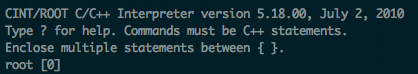
\includegraphics[width=\textwidth]{pic/cint.png}
		\begin{itemize}
		\item ROOT interactive environment is not so good for doing analysis. Both new TBrowser and command prompt environment.
		\item IPython Notebook environment. 
		\item \url{http://ipython.org/}
		\item Mathematica. Maple. Matlab. Sage.
		\item Type command. See output. Edit command. See output.
		\item Immediate inline feedback is the key. No separate windows.
		\item Save it along with output. Come back and view/re-execute later.
		\item Autocomplete. Docstring. IPython magic.
		\item inumpy
			\begin{itemize}
				\item \tiny \url{https://github.com/piti118/inumpy}
			\end{itemize}
		\end{itemize}
	\end{column}
	\begin{column}{0.5\textwidth}
		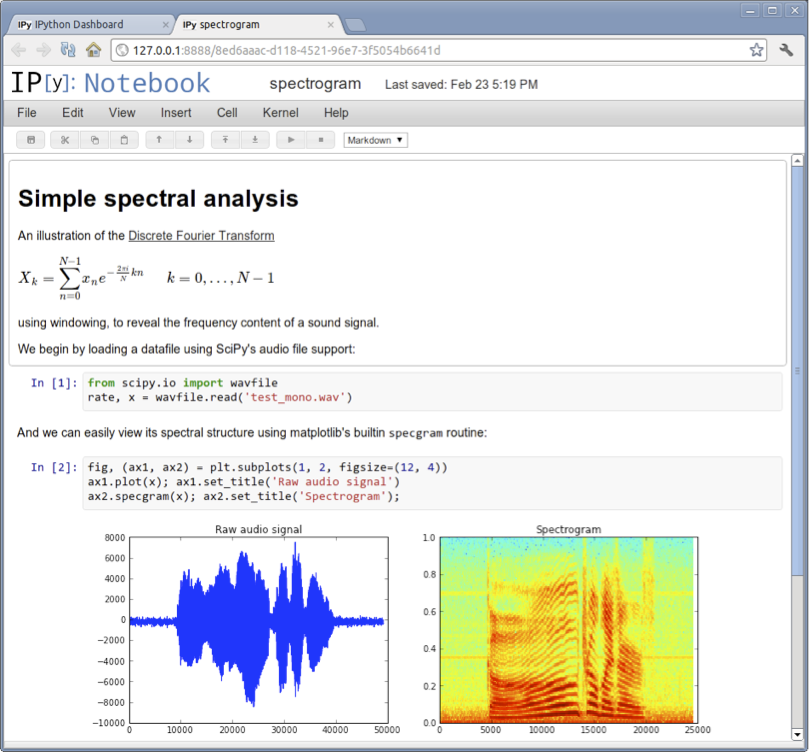
\includegraphics[width=\textwidth]{pic/ipy-notebook-spectral.png}\\
		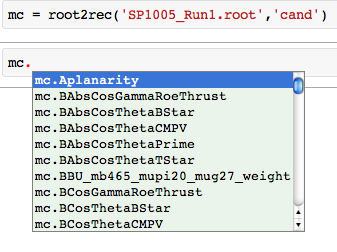
\includegraphics[width=0.8\textwidth]{pic/inumpy.png}
	\end{column}
	\end{columns}
\end{frame}

\begin{frame}[fragile, shrink=5]{Good Interactive Environment will Change Your Workflow}
\tikzstyle{decision} = [diamond, draw, fill=yellow!20, 
    text width=4.5em, text badly centered, inner sep=0pt]
\tikzstyle{block} = [rectangle, draw, fill=blue!20, 
    text width=8em, text centered, rounded corners, minimum height=2em]
\tikzstyle{blockslow} = [rectangle, draw, fill=red!20, 
    text width=8em, text centered, rounded corners, minimum height=2em]

\tikzstyle{line} = [draw, -latex']
\tikzstyle{cloud} = [draw, ellipse,fill=green!20,
    minimum height=2em]
	\begin{columns}
	\begin{column}[t]{0.5\textwidth}
		Root CINT
		\resizebox{!}{0.8\textheight}{
		\begin{tikzpicture}[node distance = 2cm, auto]
		    % Place nodes
		    \node [cloud] (start) {start};
		    \node [block, below of=start] (init) {Write Script};
		    \node [blockslow, below of=init] (load) {Load ROOT File.\\Takes a long time};
		    \node [block, below of=load] (plot) {Plot Stuff};
		    \node [decision, below of=plot] (like) {Like it?};
		    \node [decision, left of=like, node distance=4cm] (tired) {Tired?};
		    \node [cloud, below of=like, node distance=3cm] (done) {Done};
		    \node [block, left of=load, node distance=4cm] (cint) {Try Edit CINT};
		    \node [block, left of=init, node distance=4cm] (giveup) {Give Up CINT};
		    \node [cloud, below of=tired, node distance=3cm] (quit) {Quit Physics};
		    % Draw edges
		    \path [line] (start) -- (init);
		    \path [line] (init) -- (load);
		    \path [line] (load) -- (plot);
		    \path [line] (plot) -- (like);
		    \path [line] (like) -- node {Yes} (done); 
		    \path [line] (like) -- node {No} (tired);
		    \path [line] (tired) -- node {No} (cint);
		    \path [line] (tired) -- node {Yes} (quit);
		    \path [line] (cint) -- (giveup);
		    \path [line] (giveup) -- (init);
		\end{tikzpicture}
		}
	\end{column}
	\begin{column}[t]{0.5\textwidth}
		IPython + Matplotlib
		\resizebox{!}{0.8\textheight}{
		\begin{tikzpicture}[node distance = 2cm, auto]
		    % Place nodes
		    \node [cloud] (start) {start};
		    \node [block, below of=start] (init) {Write Script};
		    \node [blockslow, below of=init] (load) {Load ROOT File.\\Takes a long time};
		    \node [block, below of=load] (plot) {Plot Stuff};
		    \node [block, below left of=plot, node distance=5cm, yshift=2.5cm, text width=10em] (ipython) {Edit Cell in IPython};
		    \node [decision, below of=plot] (like) {Like it?};
		    \node [cloud, below of=like, node distance=3cm] (done) {Done};

		    % Draw edges
		    \path [line] (start) -- (init);
		    \path [line] (init) -- (load);
		    \path [line] (load) -- (plot);
		    \path [line] (plot) -- (like);
		    \path [line] (like) -- node {Yes} (done); 
		    \path [line] (like) -| node {No} (ipython);
		    \path [line] (ipython) |- (plot);
		    
		    %\path [line] (init) -- (identify);
		    %\path [line] (identify) -- (evaluate);
		    %\path [line] (evaluate) -- (decide);
		    %\path [line] (decide) -| node [near start] {yes} (update);
		    %\path [line] (update) |- (identify);
		    %\path [line] (decide) -- node {no}(stop);
		    %\path [line,dashed] (expert) -- (init);
		    %\path [line,dashed] (system) -- (init);
		    %\path [line,dashed] (system) |- (evaluate);
		\end{tikzpicture}}
		\end{column}
	\end{columns}
\end{frame}

\begin{frame}[shrink=5]{Plots looks nice by default}
	\begin{columns}
	\begin{column}{0.6\textwidth}
	\begin{itemize}	
	\item Needs tons of work to make
	ROOT plot looks OK. They changed it recently though.
	\item Gray background by default. Why? Really?
	\item Default color for COLZ.
		\begin{itemize}
			\item Legend says they are the 16 color supported 
			by color screen back then.
		\end{itemize}
	\item No transparent color!!

	\item Matplotlib. Python plotting library.
		\url{http://matplotlib.org/}
	\item Huge Gallery 
	\footnotesize{\url{ http://matplotlib.org/gallery.html}}
	\item \normalsize Extensive documentation.
	\end{itemize}
	\end{column}
	\begin{column}{0.4\textwidth}
		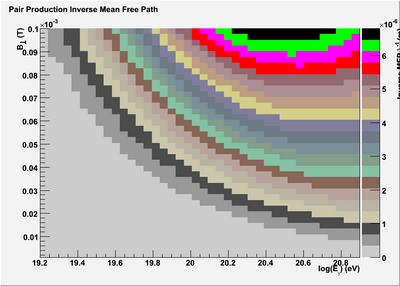
\includegraphics[width=\textwidth]{pic/default_palette_400.png}
		
		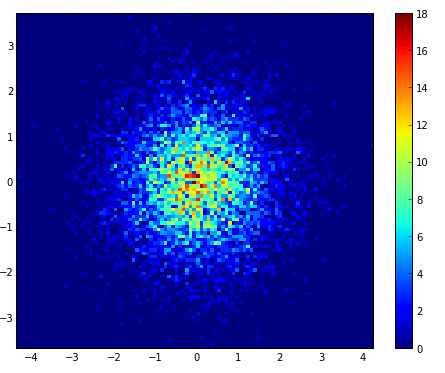
\includegraphics[width=\textwidth]{pic/hist2d-matplotlib.png}

	\end{column}
	\end{columns}
\end{frame}
\begin{frame}{Plotting syntax}
\begin{block}{Let's try to make a simple plot}
	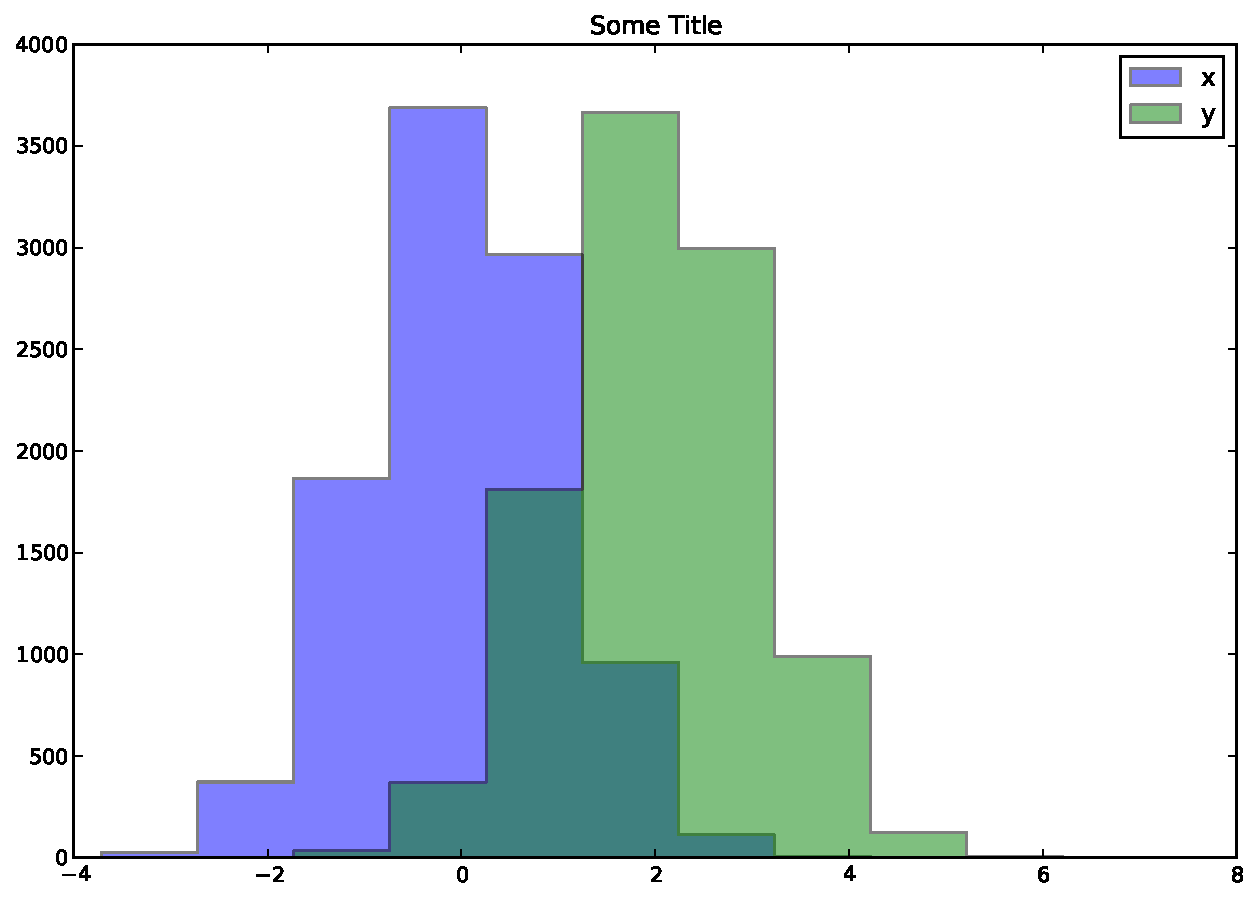
\includegraphics[width=\textwidth]{pic/mplsyntax.pdf}
\end{block}
\end{frame}

\begin{frame}[fragile, shrink=37]{Plotting Syntax}
	\begin{columns}[t]
	\begin{column}{0.5\textwidth}
	\begin{block}{ROOT. Black magic.}
	\begin{minted}[fontsize=\footnotesize, frame=single]{c++}
		tree->Draw("x");
		TH1F *xhist = (TH1F*)gPad->GetPrimitive("htemp");
		htemp->SetLineColor(kRed);
		tree->Draw("y>>h2","same");
		TH1F *yhist = (TH1F*)gPad->GetPrimitive("h2");
		yhist->SetLineColor(kBlue);
		htemp->SetTitle("Magic!!!");
		Legend* leg = new TLegend(0.1,0.7,0.48,0.9);
		leg->SetHeader("The Legend Title");
		leg->AddEntry(xhist,"x");
		leg->AddEntry(yhist,"y");
		leg->Draw();
	\end{minted}
	\end{block}
	\end{column}
	\begin{column}{0.5\textwidth}
	\begin{block}{Matplotlib. Named argument.}
		\begin{minted}[fontsize=\footnotesize, frame=single]{python}
		hist([x,y], histtype='stepfilled', label=['x','y'], 
            color=['blue','green'], alpha=0.5)
		title("Some Title")
		legend() #yep that simple.
		\end{minted}
	\end{block}
	\end{column}
	\end{columns}
	\begin{block}{Bonus}
	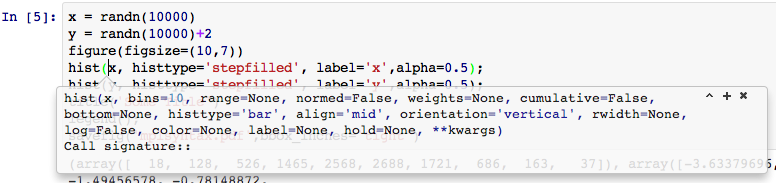
\includegraphics[width=\textwidth]{pic/ipython_doc.png}
	\end{block}
\end{frame}

\begin{frame}[fragile, shrink=5]{Multivariate Analysis and Fitting}
	\begin{itemize}
	\item Python has tons of packages to do multivariate analysis.
		\begin{itemize}
			\item Most popular one is scikit-learn
				\url{http://scikit-learn.org/}
			\item A Bunch of neural network library too.
		\end{itemize}
	\item Fitting takes advantage of Python introspection. You can ask a python function: Hey,
	what are your arguments? 
	\item This means minimizer can 
	automagically recognizes argument names as parameters. No need to repeat
	yourself.
		\begin{minted}[frame=lines]{python}
			def f(x,y,z):
			    return (x-2)**2+(y-3)**2+(z-4)**2
			m = Minuit(f)#it knows arguments are x,y,z
			m.migrad()
			print m.values #{"x":2.,"y":3.,"z":4.}
		\end{minted}
	\item Minuit and Likelihood/$\chi^2$ construction. With introspection and much more.
		\begin{itemize}
			\item \url{https://github.com/iminuit/iminuit}
			\item \url{https://github.com/iminuit/probfit}
				
		\end{itemize}
		\begin{minted}[frame=lines]{python}
			def pdf(x, mu, sigma, alpha):
			    return complicated_function(x,mu,sigma,alpha)
			lh = BinLH(pdf,data)#knows about mu, sigma, alpha
			m = Minuit(lh)
			m.migrad()
		\end{minted}
	\end{itemize}
\end{frame}

\frame{
\frametitle{Want to learn about all these?}
\begin{block}{Time and Location:}
\begin{itemize}
	\item Setup Session. 1 hour.\\ Monday Jan 28 2013 12:20pm-13:20pm Redwood C/D.
	\item Tutorial Session. 4 hour.\\ Thursday Jan 31 2013 8:30am-12:30pm Redwood C/D.
\end{itemize}
\end{block}
\begin{block}{Prepare your laptop in advance}
Visit our website for instruction. You are strongly encouraged to try to prepare your laptop before the setup session. If there is any problem, just come to Setup Session. We will try our best to help.

\url{http://piti118.github.com/babar_python_tutorial/}

\end{block}
\begin{block}{Can't attend the tutorial?}
The materials on the website is designed so that you learn it by yourself. They are all downloadable.
\end{block}
}



\end{document}
